\chapter{Modélisation des actions mécaniques}
\thispagestyle{plain} % Supprimer le header & le footer sur cette page en laissant la numérotation
\newpage

%----------------------------------------------------------------------------------------
%	Centres d'inertie
%----------------------------------------------------------------------------------------

\section{Centres d'inertie}

\exercice{Demi-circonférence}
Soit une demi-circonférence de rayon $R$, de centre $O$ et de masse linéique $\rho$.

\begin{center}
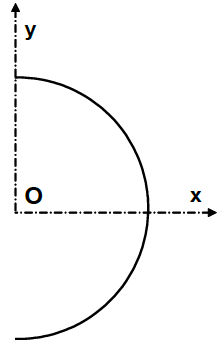
\includegraphics[scale=0.5]{png/demi-circonference.png}
\end{center}

\subsubsection{Travail demandé}
\begin{enumerate}
\item Déterminer en $O$ le torseur des actions mécaniques exercées par la
pesanteur sur la demi-circonférence.
\item Déterminer la position du centre de gravité $G$.
\end{enumerate}

\correction{ 
\begin{center}
$\overrightarrow{OG}=\frac{2.R}{\pi}.\overrightarrow{x}$
\end{center}
}
\newpage

%--------------------------------------------

\exercice{Demi-disque}
Soit un demi-disque de rayon $R$, de centre $O$ et de masse surfacique $\rho$.

\begin{center}
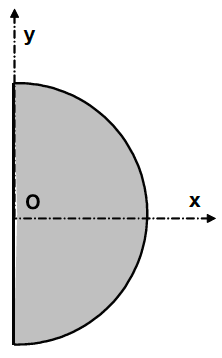
\includegraphics[scale=0.5]{png/demi-disque.png}
\end{center}

\subsubsection{Travail demandé}
\begin{enumerate}
\item Déterminer en $O$ le torseur des actions mécaniques exercées par la
pesanteur sur le demi-disque.
\item Déterminer la position du centre de gravité $G$.
\end{enumerate}

\correction{
\begin{center}
$\overrightarrow{OG}=\frac{4.R}{3.\pi}.\overrightarrow{x}$
\end{center}
}
\newpage

%--------------------------------------------

\exercice{Demi-sphère}
Soit une demi-sphère de rayon $r$, de centre $O$ et de masse volumique $\rho$.

\begin{center}
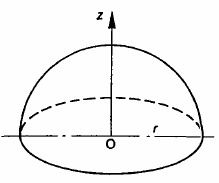
\includegraphics[scale=0.7]{png/demi-sphere.png}
\end{center}

\subsubsection{Travail demandé}
\begin{enumerate}
\item Déterminer en $O$ le torseur des actions mécaniques exercées par la
pesanteur sur la demi-sphere.
\item Déterminer la position du centre de gravité $G$.
\end{enumerate}

\correction{ 
\begin{center}
$\overrightarrow{OG}=\frac{4.R}{3.\pi}.\overrightarrow{z}$ (à vérifier)
\end{center}
}
\newpage

%--------------------------------------------

\exercice{Cône de révolution plein et homogène}
Soit un cône de révolution plein et homogène de hauteur $h$.\\

\begin{center}
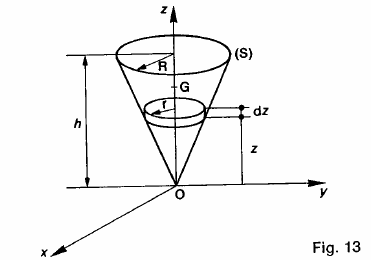
\includegraphics[scale=0.6]{png/cone.png}
\end{center}

\subsubsection{Travail demandé}
Déterminer son centre de gravité.

\correction{ 
\begin{center}
$\overrightarrow{OG}=\frac{3}{4}.h.\overrightarrow{z}$
\end{center}
}
\newpage

%--------------------------------------------

\exercice{Centres d'inertie}
\textit{Remarque : C'est Euler qui a introduit le terme de centre d'inertie à la place de celui de centre de gravité.}
\begin{enumerate}
\item Déterminer le centre d’inertie du secteur circulaire d’angle $2\alpha$ d’une couronne de rayon intérieur $r$ et de rayon extérieur $R$, supposée homogène.

\begin{center}
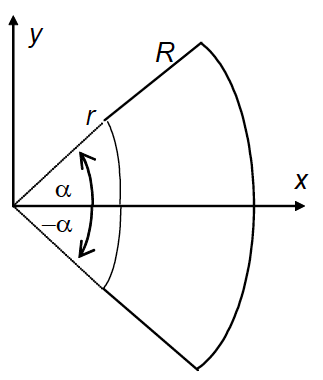
\includegraphics[scale=0.5]{png/CI1.png}
\end{center}

\item Déterminer la position du centre d'inertie de la surface hachurée $ABC$, la courbe $AB$ étant un quart de cercle de rayon $R$.

\begin{center}
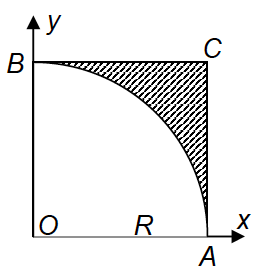
\includegraphics[scale=0.5]{png/CI2.png}
\end{center}
\end{enumerate}

\correction{ 
\begin{enumerate}
\item $\overrightarrow{OG}=\frac{2}{3}.\frac{R^2+R.r+r^2}{R+r}.\frac{1}{\alpha}.\sin(\alpha).\overrightarrow{x}$
\item Théorème de superposition + résultat de l'exercice précédent avec $\alpha=\frac{\pi}{4}$.
\end{enumerate}
}
\newpage

%--------------------------------------------

\exercice{Centre de gravité du plane}
La plaque plane ci–dessous a une épaisseur de $1 mm$. Elle est constituée en alliage d'aluminium et comporte deux trous circulaires et un trou oblong (voir dessin).

\begin{center}
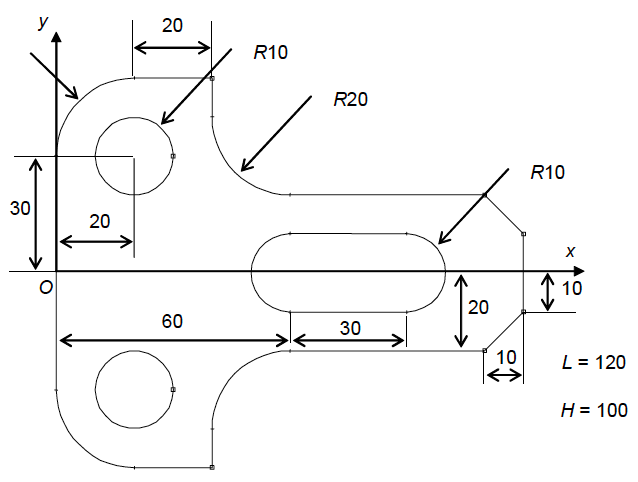
\includegraphics[scale=0.5]{png/piece_alu.png}
\end{center}

\subsubsection{Travail demandé}
Déterminer la position du centre de gravité de cette plaque.


\correction{ 
\[ \overrightarrow{OG}=44,997.\overrightarrow{x}  \text{(en mm)}\]
}
\newpage

%----------------------------------------------------------------------------------------
%	Modélisations des actions mécaniques
%----------------------------------------------------------------------------------------

\section{Modélisations des actions mécaniques}

\exercice{Panneau indicateur}
Un panneau indicateur, figure ci-dessous, est soumis à son propre poids et à
l’action du vent sur sa partie rectangulaire. Le poids linéique des montants $OA$ et $AB$ est $\overrightarrow{q} = –q.\overrightarrow{y}$. Le poids du panneau $CDEF$ est $\overrightarrow{P} = – M.g.\overrightarrow{y}$. L’action du vent sur $CDEF$ est représentée par une densité surfacique d’efforts $\overrightarrow{p} = –p.\overrightarrow{z}$ ($p$ constant).

\subsubsection{Données géométriques}
\begin{center}
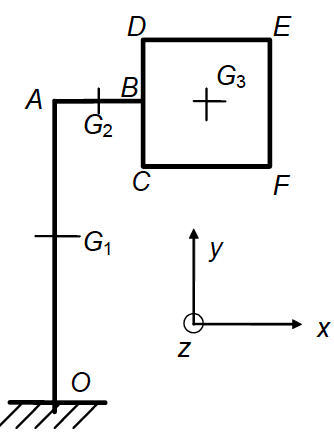
\includegraphics[scale=0.5]{png/panneau.png}
\end{center}
On donne les valeurs numériques suivantes :
\begin{description}
\item $OA = 7,5 m$
\item $AB = 3 m$
\item $DC = 3 m$
\item $DE = 4 m$
\item $q = 750 N/m$
\item $p = 500 N/m^2$
\item $Mg = 7000 N$
\end{description}

\subsubsection{Travail demandé}
Calculer le torseur d’action mécanique en O du sol sur cette structure.

\correction{ 
\begin{center}
$T_O = \left\{
\begin{array}{rcl}
	14875\overrightarrow{y} + 6000\overrightarrow{z} \\
	45000\overrightarrow{x} - 30000\overrightarrow{y} + 38375\overrightarrow{z}
\end{array}\right.$ en $O$
\end{center}
}
\newpage

%--------------------------------------------

\exercice{Une toiture bien solicitée}

Une toiture est soumise à l’action du vent sur l’un de ses versants et à l’action de la neige sur l’autre. Les actions des murs sur la charpente sont telles que seuls les déplacements en $A$ suivant $\overrightarrow{x}$ et $\overrightarrow{y}$, et en $B$ suivant $y$ soient bloqués. On négligera les effets de bord suivant $\overrightarrow{z}$ dans cet exercice, c’est–à–dire que l’on considérera une épaisseur unité ($1 m$) suivant $\overrightarrow{z}$.\\\\
On suppose que l’épaisseur constante de la neige sur la toiture est $e = 20 cm$, et que l’action du vent est linéaire suivant la cote de la toiture avec une valeur maximale sur la faîtière (en $C$) égale à $1 kN/m^2$, le glisseur unitaire est orthogonal à la toiture (voir figure).

\begin{center}
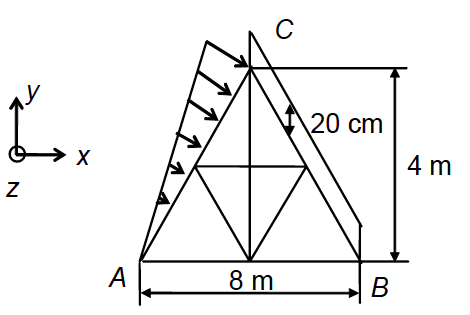
\includegraphics[scale=0.5]{png/toiture.png}
\end{center}

\subsubsection{Travail demandé}
Déterminer les actions mécaniques de la toiture sur le mur.

\correction{ 
\begin{center}
$T_A = \left\{
\begin{array}{rcl}
	-2000\overrightarrow{x} + 2667\overrightarrow{y} \\
	\overrightarrow{0}
\end{array}\right.$ en $A$\\
$T_B = \left\{
\begin{array}{rcl}
	7333\overrightarrow{y}\\
	\overrightarrow{0}
\end{array}\right.$ en $B$
\end{center}
}
\newpage

%--------------------------------------------

\exercice{Dalle de béton}

Soit une surface plane rectangulaire subissant une répartition surfacique $\overrightarrow{P}$ constante suivant $\overrightarrow{x}$ telle que : $\overrightarrow{P}=-(\frac{P_m}{L}.y+P_0).\overrightarrow{z}$

\begin{center}
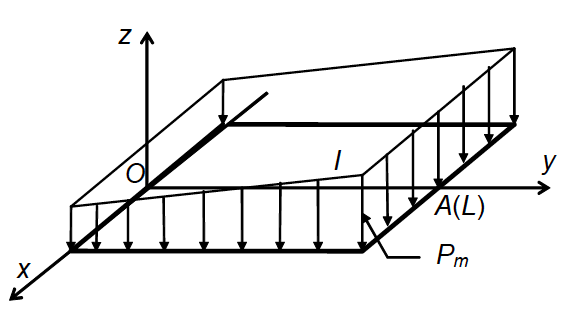
\includegraphics[scale=0.5]{png/dalle.png}
\end{center}

\subsubsection{Travail demandé}
\begin{enumerate}
\item Calculer le torseur en $O$ représentant cette action répartie.
\item Déterminer la position $I$ du glisseur équivalent à cette répartition.
\end{enumerate}

\correction{ 
\begin{enumerate}
\item \[T_O = \left\{
\begin{array}{rcl}
	\overrightarrow{R}=-(\frac{P_m}{2}+P_0).L.l.\overrightarrow{z} \\
	\overrightarrow{M_0}=-(\frac{P_m}{3}+\frac{P_0}{2}).L^2.l.\overrightarrow{x}
\end{array}\right. \text{en O}\]
\end{enumerate}
}
\newpage

%--------------------------------------------

\exercice{Chaînette}

Déterminer la forme d'un fil homogène, parfaitement souple, de section uniforme, en équilibre sous l'action de son poids et des actions des points de fixation $O_1$ et $O_2$ des extrémités. La masse linéique sera notée $\mu$.

\begin{center}
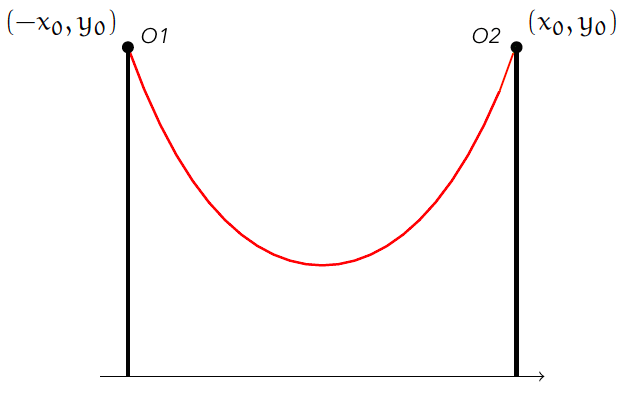
\includegraphics[scale=0.5]{png/chainette.png}
\end{center}

\newpage